\chapter{\textit{Análise de Controle}}

Agora que já definimos o comportamento dinâmico de um quadricóptero, nesse capítulo vamos entender como podemos modelar um sistema de controle que seja efetivo no controle das nossas variáveis de interesse, assim passaremos brevemente sobre a teoria de controle e os passos que devemos seguir para montarmos o sistema de controle do quadricóptero em questão. Sendo assim, como este trabalho tem o intuito de analisar o mini drone Mambo da parrot, vamos partir do príncipio que não podemos fazer nenhuma modificação no modelo físico do drone para melhorar sua performance de controle, por exemplo, não podemos adicionar mais um sensor. Então para montarmos nosso problema de controle, precisamos analisar as características do nossa planta, o mini drone Mambo.

\section{Sistemas de Controle}

Podemos definir um sistema como uma coleção de componentes interagindo entre si, exemplos disso podem ser um carro, um motor, ou até mesmo o corpo humano. Sendo assim um sistema pode ser caracterizado por duas propriedades (adicionar citação):

1. Interrelação entre os componentes contidos no sistema.

2. Limites que separam os os componentes dentro do sistema e os que estão fora dele.

Sobre o item 2, quando falamos dos limites que determinam um sistema, esses limites podem ser reais ou imaginários e mutáveis, podendo ser redefinidos a qualquer momento da análise do sistema,por exemplo dividindo um sistema grande em subsistemas, que podem ser analisados separadamente, ou agrupando dois subsistemas em um único sistema.

Assim, quando lidamos com sistemas, nosso maior interesse é nos efeitos que interações externas ao sistema afetam seu comportamento. Na figura abaixo temos a representação de um sistema, onde definimos as interações externas, como entrada, e o resultado da sua interação com o sistema, de saída. O que chamamos de sáida também pode ser chamado de estado do sistema, e pode ser descrito por suas \textit{variáveis de estado}, que em conjunto com a entrada do sistema nos permite determinar seu estado futuro, o que se encaixa na definicão de um sistema dinâmico. Logo quando tratamos de sistemas dinâmicos queremos especificar as entradas do sistema, que o façam se comportar de alguma maneira específica e obtemos isso atráves do controlador, sendo assim quando falamos que nosso interesse está nos efeitos que as entradas causam no estado do sistema, estamos dizendo que queremos controlar a saída do sistema, gerando uma entrada adequada que faça que o sistema e suas váriaveis de estado se comportarem de determinada maneira de interesse. A relação entre o sistema e o controlador é chamada de sistema de controle.

Podemos ter sistemas de controle com feedback e sistemas de controle sem feedeback, estes são chamados respectivamente se sistema de controle de malha fechada e de malha aberta, se observamos as imagens, podemos ver o porquê, um sistema de controle de malha fechada usa feedback para ajustar a ação de controle com base na diferença entre a saída desejada e a saída real, já um sistema de controle de malha aberta a ação de controle é determinada com base na entrada desejada, sem considerar a saída real do sistema.

Nesses sistemas de controle, sempre temos:
- Um processo a ser controlado,o que podemos chamar de planta,
- A váriavel de controle da planta, que chamamos de entrada,
- A variável a ser controlada pela planta, que chamamos de saída,
- O valor de entrada de referência, que nos diz qual a saída desejada,
- O controlador, que a partir do entrada de referência gera o input necessário para que a planta tenha a saída desejada.

O que difere o sistema de malha fechada para o de dmalha aberta são os seguintes componentes:

- Ponto de junção, onde o sinal de saída medido é subtraído do sinal de referência de entrada para medir o sinal de erro.

- Feedback iterativo, onde o sinal de saída é medido com um sensor e retornado para o ponto de junção.



\begin{figure}[H]
	\centering
	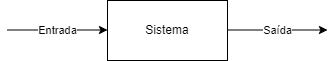
\includegraphics[width=1\textwidth]{controle-sistema-simples.png}
	\caption{Representação de um sistema}
	\centering
	\label{Representação de um sistema}
\end{figure}

\begin{figure}[H]
	\centering
	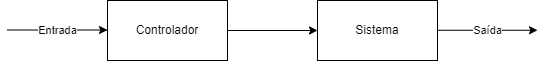
\includegraphics[width=1\textwidth]{controle-sistema-open.png}
	\caption{Representação de um sistema de malha aberta}
	\centering
	\label{Representação de um sistema de malha aberta}
\end{figure}

\begin{figure}[H]
	\centering
	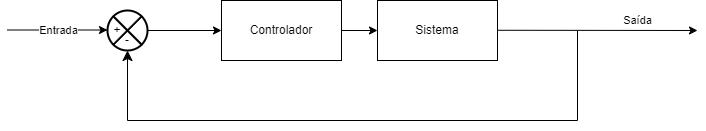
\includegraphics[width=1\textwidth]{controle-sistema-closed.png}
	\caption{Representação de um sistema de malha fechada}
	\centering
	\label{Representação de um sistema de malha fechada}
\end{figure}

\subsection*{Sistema de controle de um quadricóptero}

Na seção anterior, definimos o que é um sistema de controle de forma simples e genérica, com isso em mente agora vamos definir o sistema de controle para um quadricóptero. Nos capítulos anteriores, abordamos as características do quadricóptero que vamos utilizar, sendo assim, conseguimos determinar nosso problema de controle da forma abaixo:

- Planta, que é o modelo dinâmico do nosso quadricóptero;

- Controlador, que é o algoritimo usado para calcular o comando dos motores para que nosso drone atinja o mais precisamente possível a manobra/posição desejada no espaço 3d;

- Sensores, que vão nos ajudar a medir nossas variáveis de estado que serão comparadas com o nosso ponto de referência.


\begin{figure}[H]
	\centering
	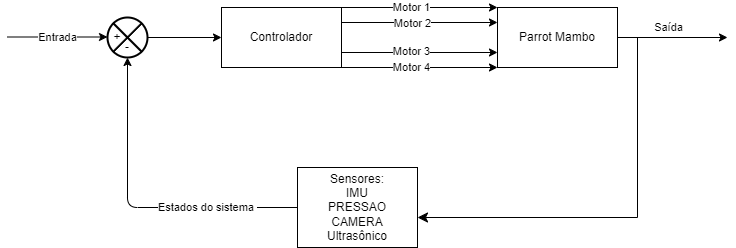
\includegraphics[width=1\textwidth]{controle-sistema-quadricoptero.png}
	\caption{Representação do sistema de controle do Quadricóptero}
	\centering
	\label{Representação do sistema de controle do Quadricóptero}
\end{figure}

Nesse momento nosso foco está no controlador, sendo assim é importante notarmos que esse é um sistema subatuado,pois temos 4 atuadores(motores) e 6 graus de liberdade, o que significa que como nâo temos um atuador para cada movimento nós sabemos que algumas direções não são controladas em momento algum, por exemplo o drone não é capaz de se mover para esquerda sem antes fazer um rolamento, ou para trás e para frente sem antes fazer uma arfagem. Dessa forma, nosso objetivo é superar esse problema do sistema subatuado desenvolvendo um controlador que combina rotações e a propulsão gerada para atingir os objetivos.

Nesse sentido, precisamos saber como gerar propulsão, rolamento, guinada, arfagem com apenas 4 motores e porque a direção de giro das hélices nos permite desacoplar esses movimentos.
A configuração dos drones, geralmente é feita utilizando uma combinação de um par de hélices girando no sentido horário e outro no anti-horário, pois como sabemos, quando as hélices giram, além de produzirem sustentação, elas geram torque na direção oposta de rotação. Assim se todas estivessem girando na mesma direção o drone iria girar incontrolavelmente. Dessa forma podemos controlar esses 4 movimentos de forma independente, da seguinte forma:

- Controle de Propulsão - Todas as hélices girando com a mesma velocidade.

- Controle de Guinada - Para rotacionar o drone em torno do seu eixo vertical, a velocidade de um dos pares de hélices(horário ou anti-horário) tem que ser ajustada. Por exemplo aumentando a velocidade do par de hélices girando no sentido horário e ao mesmo tempo diminuindo a velocidade no sentido anti-horário vai gerar um torque que não vai ser completamente cancelado, fazendo o drone dar uma guinada, enquanto mantém sua altura.

- Controle de Rolamento e Arfagem - Para um rolamento(inclinação para direita ou para esquerda), ou arfagem(inclinação para frente ou para trás). Tem-se que ajudater os pares opostos de hélices. Por exemplo, para uma arfagem para frente, o par de trás aumenta de velocidade e o par da frente diminui a velocidade.

Sendo assim esses são os quatro movimentos que podemos controlar independentemente, e o comando para os motores será uma mistura da propulsão, guinada, rolagem e arfagem necessária.

SA - Sentido horário
SAH - Sentido anti-horário

\begin{table}[h!]
	\centering
	\begin{tabular}{|c|c|c|c|}
	\hline
	{\textbf{Command}} & \multicolumn{3}{c|}{\textbf{Cross Configuration}} \\ \cline{2-4}
	 & \textbf{Estado da Velocidade} & \textbf{PAR 1, 3} & \textbf{PAR 2, 4} \\ \hline
	\textbf{Pairar (H)} & $\omega_{m1} = \omega_{m3}$ & $\omega_{m2} = \omega_{m4}$ & \textbf{PAR 1, 3 = PAR 2, 4} \\ \hline
	\textbf{SH Arfagem} & $\omega_{m1} > \omega_{m3}$ & $\omega_{m2} > \omega_{m4}$ & N/A \\ \hline
	\textbf{SH Rolagem} & $\omega_{m1} < \omega_{m3}$ & $\omega_{m2} > \omega_{m4}$ & N/A \\ \hline
	\textbf{SH Guinada} & $\omega_{m1} = \omega_{m3}$ & $\omega_{m2} = \omega_{m4}$ & \textbf{Par 1, 3} < \textbf{ Par 2, 4} \\ \hline
	\textbf{SAH Arfagem} & $\omega_{m1} < \omega_{m3}$ & $\omega_{m2} < \omega_{m4}$ & N/A \\ \hline
	\textbf{SAH Rolagem} & $\omega_{m1} > \omega_{m3}$ & $\omega_{m2} < \omega_{m4}$ & N/A \\ \hline
	\textbf{SAH Guinada} & $\omega_{m1} = \omega_{m3}$ & $\omega_{m2} = \omega_{m4}$ & \textbf{Par 1, 3} > \textbf{ Par 2, 4}\\ \hline
	\end{tabular}
	\caption{Tabela de Comandos para Configuração Cross}
	\label{tab:control-config}
	\end{table}

	\begin{figure}[h]
		\centering
		\begin{equation*}
			\begin{aligned}
				\text{Motor}_{\text{frontal direito}} & = \text{Propulsão} + \text{Guinada}_{\text{cmd}} + \text{Arfagem}_{\text{cmd}} + \text{Rolagem}_{\text{cmd}} \\
				\text{Motor}_{\text{frontal esquerdo}} & = \text{Propulsão} + \text{Guinada}_{\text{cmd}} + \text{Arfagem}_{\text{cmd}} - \text{Rolagem}_{\text{cmd}} \\
				\text{Motor}_{\text{traseiro direito}} & = \text{Propulsão} + \text{Guinada}_{\text{cmd}} + \text{Arfagem}_{\text{cmd}} + \text{Rolagem}_{\text{cmd}} \\
				\text{Motor}_{\text{traseiro esquerdo}} & = \text{Propulsão} + \text{Guinada}_{\text{cmd}} + \text{Arfagem}_{\text{cmd}} - \text{Rolagem}_{\text{cmd}}
			\end{aligned}
		\end{equation*}
		\caption{Algoritimo dos motores do drone}
	\end{figure}

Como já comentamos, os movimentos para trás, pra frente, para direita e para esquerda, não são atuados, e nos movimentos nessas direções, primeiro rotacionando o drone numa atitude onde nosso vetor de propulsão está parcialmente na direção da gravidade e parcialmente na direção que escolhemos ir, para acelerarmos o drone naquela direção, sendo assim para manter altura durante essa manobra, precisamos aumentar a propulsão de forma que ela continue a cancelar a ação da gravidade.

\subsection*{Controlador de Voo Pairado}

Com o que já vimos nos capítulos anteriores, agora podemos desenvolver nosso controlador. Para isso, vamos utilizar a missão mais simples de voo que é um voo pairado, ou seja, queremos que nosso drone levante voo e não se mova signficativamente no plano X,Y. Assim sendo temos que controlar a posição do drone no plano X,Y,Z, a partir das nossas quatro váriaveis controláveis independentemente, rolagem, guinada, arfagem e propulsão.

A principio para um voo pairado, podemos pensar em um controlador de altitude,  que tem como entrada a altitude, aumentando ou diminuindo a propulsão até atingir a altitude necessária, no formato abaixo:

\begin{figure}[H]
	\centering
	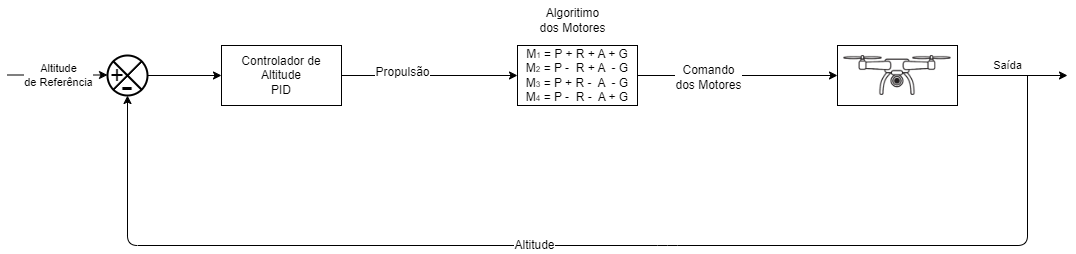
\includegraphics[width=1\textwidth]{flightControlSystem-controller-manbo-altitude.png}
	\caption{Sistema de controle utilizando apenas Propulsão para Controle de Altitude}
	\centering
	\label{Sistema de controle utilizando apenas Propulsão para Controle de Altitude}
\end{figure}


\begin{figure}[H]
	\centering
	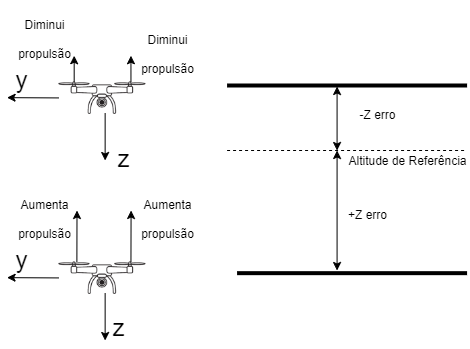
\includegraphics[width=1\textwidth]{flightControlSystem-controller-manbo-altitude-work.png}
	\caption{Funcionamento de um sistema de Controle utilizando apenas Propulsão para Controle de Altitude}
	\centering
	\label{Funcionamento de um sistema de Controle utilizando apenas Propulsão para Controle de Altitude}
\end{figure}

Em mundo ideal, sem nenhuma perturbação, como o vento, considerando que todos os motores estão perfeitamente calibrados,e que o aumento da propulsão vai gerar apenas aumento na velocidade em Z, este seria um ótimo controlador, mas no mundo real essa não é a situação que temos, geralmente temos perturbações naturais como rajadas de vento, ou neve, os motores podem estar descalibrados entre si então um aumento na propulsão pode causar aumento na velocidade horizontal. Ou seja nosso sistema ainda não está preparado para lidar com o mundo real, por exemplo uma rajada de vento pode causar uma mudança no ângulo de rolagem ou arfagem fazendo com que o aumento da propulsão cause aumento na velocidade horizontal do drone o fazendo se movimentar no plano XY descontroladamente, se afastando do ponto de partida, então o drone atingiria a altitude necessária, que é o objetivo, mas se movimentaria no plano XY, que não é o objetivo. Assim, diferente do que pode-se pensar inicialmente, temos que controlar nossas quatro váriaveis independentemente. E teríamos um sistema de controle como o abaixo.


\begin{figure}[H]
	\centering
	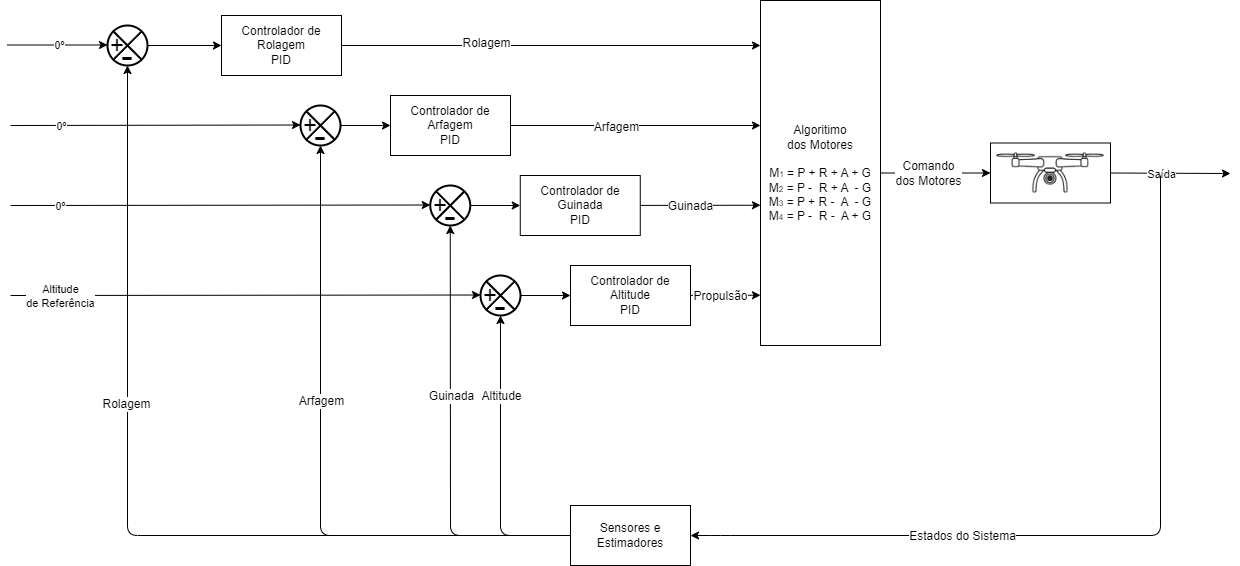
\includegraphics[width=1\textwidth]{flightControlSystem-controller-manbo-4-controllers.png}
	\caption{Sistema de Controle utilizando todas as variáveis controláveis}
	\centering
	\label{Sistema de Controle utilizando todas as variáveis controláveis}
\end{figure}

O que considera todas as nossa variáveis controláveis, mas se observarmos com atenção e fizermos o exercício de considerar uma rajada de vento lateral temos que:


- \( t_0 \) - Drone está fazendo voo pairado (\(\phi = 0\)), (\(\psi = 0\)) e (\(\theta = 0\)), (\(\dot{\phi} = 0\)), (\(\dot{\psi} = 0\)) e (\(\dot{\theta} = 0\)), (\(\dot{x} = 0\)), (\(\dot{y} = 0\)), (\(\dot{z} = 0\)), \( Z > 0 \), \( X = 0 \), \( Y = 0 \);

- \( t_1 \) - Drone recebe rajada de vento (\(\phi = 0\)), (\(\psi = 0\)) e (\(\theta > 0\)), (\(\dot{\phi} = 0\)), (\(\dot{\psi} = 0\)) e (\(\dot{\theta} > 0\)), (\(\dot{x} > 0\)), (\(\dot{y} = 0\)), (\(\dot{z} < 0\)), \( Z > 0 \), \( X > 0 \), \( Y = 0 \).

- \( t_2 \) - Drone ajusta ângulos de guinada, arfagem e rolagem e altitude (\(\phi = 0\)), (\(\psi = 0\)) e (\(\theta = 0\)), (\(\dot{\phi} = 0\)), (\(\dot{\psi} = 0\)) e (\(\dot{\theta} = 0\)), (\(\dot{x} = 0\)), (\(\dot{y} = 0\)), (\(\dot{z} = 0\)), \( Z > 0 \), \( X > 0 \), \( Y = 0 \);

Assim, podemos notar que, apesar de ajustarmos nossas quatro varráveis atuadas e conseguirmos ter um voo pairado. Caso esse ciclo se repetisse, a cada rajada de vento a posição \( X \) iria aumentar devido à aceleração nesse eixo causada pelo breve instante entre a rolagem (\(\theta > 0\)) e a correção do ângulo (\(\theta = 0\)). Ou seja esse sistema de controladores que elaboramos ainda é insuficiente para o nosso objetivo que é realizar um voo pairado e que apesar das perturbações externas faça o voo sem se afastar do local de decolagem.


\begin{figure}[H]
	\centering
	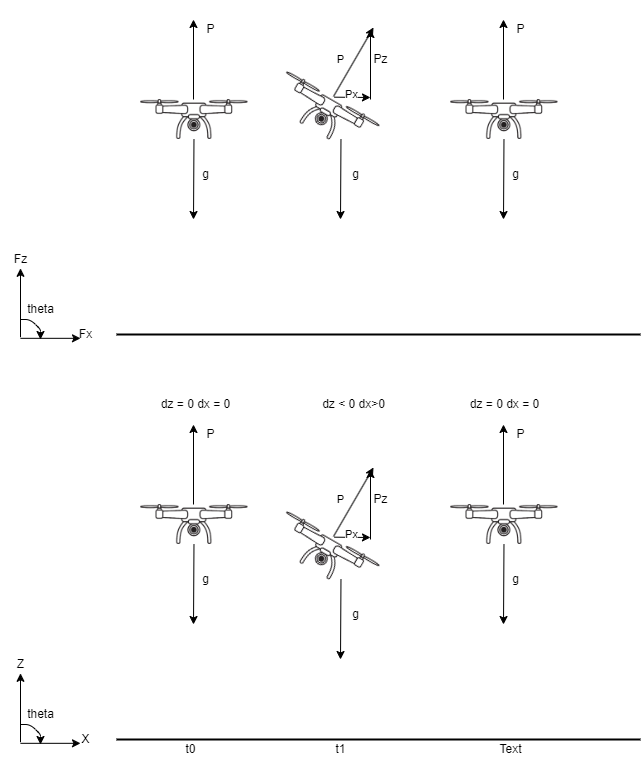
\includegraphics[width=1\textwidth]{flightControlSystem-controller-manbo-altitude-work-wind.png}
	\caption{Drone sobre influência de rajada de vento controlando apenas 4 váriaveis atuadas}
	\centering
	\label{Drone sobre influência de rajada de vento controlando apenas 4 váriaveis atuadas}
\end{figure}

Ou seja, assumir que para um voo pairado nossos ângulos de guinada, arfagem e rolagem tem que ser zero, não é uma boa interpretação para o nosso sistema de controle então, mas também não queremos fixar ângulos específicos de arfagem e rolagem, na verdade nosso objetivo está em controlar a posição em relação ao solo, plano X,Y.

Assim, podemos adicionar um controlador de posição que vai conter controladores de arfagem e rolagem para manter a posição em X,Y. Nesse sentido, os controladores de arfagem e rolagem internos ao controlador de posição vão calcular a entrada de referência para os controladores de arfagem e rolagem. Logo temos o loop externo, que gera os sinais de referência de arfagem e rolagem para o loop interno, sendo importante notar que o ângulo de guinada também vai ser utilizado no controlador de posição. Os erros de posição X-Y são expressos em relação ao referencial do ambiente, mas os ângulos de arfagem e rolagem são expressos em relação ao referencial do drone. Isso significa que um movimento nas direções X e Y do mundo pode ser obtido através da arfagem e rolagem apenas conhecendo o ângulo de guinada, pois ele é necessário para o controlador de posição fazer a conversão do referencial X-Y do drone para o referencial do ambiente.
 

\begin{figure}[H]
	\centering
	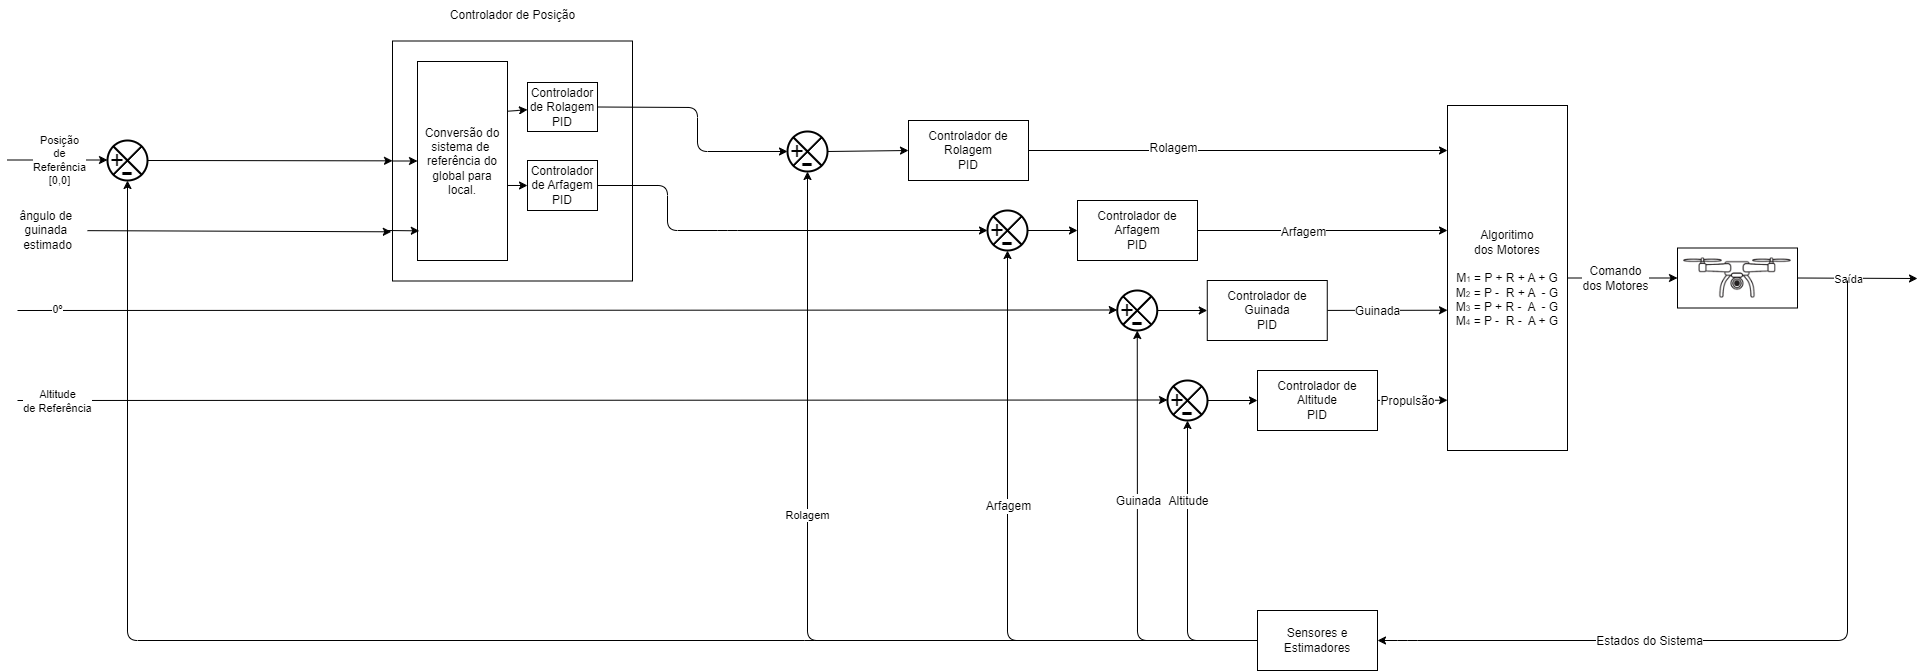
\includegraphics[angle=90,width=0.5\textwidth]{flightControlSystem-controller-manbo-6-controllers-complete.png}
	\caption{Sistema de controle de um quadricóptero para Voo Pairado}
	\centering
	\label{Sistema de controle de um quadricóptero para Voo Pairado}
\end{figure}

Outro ponto importante de notarmos no nosso sistema, é que apesar de termos idealizado ele pensando em um voo pairado, ele pode ser útil para outros objetivos, como por exemplo navegar para uma posição específica e pousar. O que é importante nesse controlador que idealizamos é que podemos controlar os 6 graus de liberdade do drone.

Podemos inclusive lembrar do exercício que fizemos acima, sobre os instantes e teríamos uma mudança em \( t_2 \) e no próximo instante estaríamos na posição original no plano XY.

- \( t_2 \) - Drone ajusta ângulos de guinada, arfagem e rolagem e altitude e posição em x (\(\phi = 0\)), (\(\psi = 0\)) e (\(\theta = 0\)), (\(\dot{\phi} = 0\)), (\(\dot{\psi} = 0\)) e (\(\dot{\theta} < 0\)), (\(\dot{x} > 0\)), (\(\dot{y} = 0\)), (\(\dot{z} = 0\)), \( Z > 0 \), \( X > 0 \), \( Y = 0 \);

- \( t_3 \) - Drone na posição original, pairando sobre o ponto de decolagem (\(\phi = 0\)), (\(\psi = 0\)) e (\(\theta = 0\)), (\(\dot{\phi} = 0\)), (\(\dot{\psi} = 0\)) e (\(\dot{\theta} = 0\)), (\(\dot{x} = 0\)), (\(\dot{y} = 0\)), (\(\dot{z} = 0\)), \( Z > 0 \), \( X = 0 \), \( Y = 0 \);
%---------------------------------------------------------------------
% INDICE REMISSIVO
%---------------------------------------------------------------------
\phantompart
\printindex
%---------------------------------------------------------------------
